\subsection{Overall Dataset Composition}


The BrainScape dataset include four common anatomical MRI contrasts i.e. T1-weighted (T1w), T2-weighted (T2w), 
gadolinium-enhanced T1-weighted (T1Gd), and fluid-attenuated inversion recovery (FLAIR).
Furthermore it integrates a total of \NumDatasets\ datasets from diverse open source repositories and individual research studies. 
After quality-control and visual inspection (e.g., excluding MRIs with artifacts, corrupted and poor quality scans), 
\TotalNumSubjects\ unique subjects remain in the database, yielding \TotalNumMRIs\ MRI scans overall. 

Among these, \TotalTOneMRIs\ are T1w, \TotalTTwoMRIs\ are T2w, \TotalTOneGdMRIs\ are T1Gd, and \TotalFlairMRIs\ are FLAIR. 
As summarized in Table~\ref{TableMriModDistribution}, the distribution of modalities is uneven, 
with T1w scans representing a larger share of the total MRIs. 
Yet, the inclusion of T2w and FLAIR scans extends the framework's utility to 
applications where multi-contrast data are essential (e.g., lesion analysis, tissue segmentation).


% \begin{table}[htbp]
%     \centering
%     \caption{High-Level MRI Statistics.}
%     \label{TableMainSummary}
%     \begin{tabular}{lc}
%         \hline
%         \textbf{Statistic} & \textbf{Value} \\
%         \hline
%         Datasets Included & \NumDatasets\ \\
%         Subjects (After QC) & \TotalNumSubjects\ \\
%         Total MRI Scans & \TotalNumMRIs\ \\
%         \hline
%     \end{tabular}
% \end{table}

\begin{table}
    \centering
    \begin{threeparttable}
        \caption{MRI Modality Distribution.}
        \label{TableMriModDistribution}
        \begin{tabular}{lcc}
            \toprule
            \textbf{Modality} & \textbf{Count} & \textbf{(\% of Total)} \\
            \midrule
            T1w    & \TotalTOneMRIs\    & \TOnePercent \\
            T2w    & \TotalTTwoMRIs\    & \TTwoPercent \\
            T1Gd    & \TotalTOneGdMRIs\    & \TOneGdPercent \\
            FLAIR  & \TotalFlairMRIs\   & \FlairPercent \\
            \bottomrule
        \end{tabular}
    \end{threeparttable}   
\end{table}

    
As shown in Table~\ref{TableMriModDistribution}, T1w scans are substantially more common than T2w, T1Gd and FLAIR scans.
Among the \NumDatasets\ datasets included in BrainScape, only one dataset (BRATS) provides T1Gd MRI scans. 
T2w MRI scans are available in \NumDatasetsWithTTwoScans\ datasets, 
FLAIR scans in \NumDatasetsWithTFlairScans\, 
and T1w scans in \NumDatasetsWithTToneScans\ datasets.
On the other hand, the number of sessions per subject also varies, 
ranging from a single scan per subject to multiple scans per subject. BrainScape dataset 
retains session information and the original dataset structures, ensuring flexibility 
for downstream analyses. For complete details of each individual dataset and the available
MRI modalities, refer to the Supplementary Material (Table~\ref{suppDataTable}).

Since T1w scans are more common than other modalities, 
analyses relying primarily on T2w, T1Gd, or FLAIR scans may include fewer subjects. 
However, the availability of multimodal MRI scans remains valuable for specialized clinical studies or advanced modeling tasks such as lesion segmentation. 
Researchers can leverage BrainScape's flexibility to utilize the entire dataset or a subset of the dataset, depending on the specific requirements of the study.

\begin{figure}[ht]
    \centering
    \includegraphics[width=\linewidth]{figures/example_multimodal_mri.png} 
    \caption{
        Multimodal MRIs of three subjects from different datasets with each subject having T1w, T2w, and FLAIR modalities. 
        The vertical axis (Y-axis) lists each subject by its source dataset identifiers (detailed in the Supplementary Material), 
        while the horizontal axis shows axial, coronal, and sagittal slices for each modality. 
        Here, the subject from the ``QTAB'' dataset is a 10-year-old female, 
        the subject from ``MPLMBB'' is a male aged between 65-70, 
        and the subject from ``ARCD'' is a 40-year-old male with a stroke. 
    }
    \label{fig:ExampleMultimodal}
\end{figure}

The MRI scans aggregated in the BrainScape dataset originate from scanners with diverse hardware, manufacturers, and magnetic field strengths.
Among the \TotalNumMRIs\ MRIs included, MRI scanner metadata was available for 24508 scans (52.61\%), 
while scanner information for the remaining 22075 scans (47.39\%) was missing (see Supplementary Table \ref{tab:scanner_info}). 
Furthermore, among the 24508 MRIs with scanner information, 22089 MRIs had magnetic field strengths information available.
MRI data originated primarily from three major manufacturers (Siemens, Philips, and GE), 
with Siemens scanners being the most prevalent across all modalities. 
The dataset predominantly includes 3.0 Tesla (T) MRI scanners (18147 scans), followed by 1.5T (2584 scans), 
4.0T (1301 scans), and a small subset from 7.0T scanners (57 scans). 
The BrainScape dataset contains scans from a wide range of manufacturers, models, and field strengths, 
mirroring the variability seen in clinical and research imaging. 
This diversity makes BrainScape dataset an excellent resource for training AI models that are both robust and generalizable.
Additionally, scanner metadata, including the manufacturer name, model details, and field strength information, is stored in the BrainScape JSON record.

Figure~\ref{fig:ExampleMultimodal} illustrates how BrainScape integrates multimodal MRI data 
from diverse heterogeneous datasets, with varying participant demographics and clinical profiles. 
Our framework effectively combines these heterogeneous datasets and enables researchers 
to examine both healthy individuals and those with specific conditions (such as stroke). 
Moreover, BrainScape preserves the demographic and clinical metadata, allowing researchers 
to readily filter or subgroup images by attributes like age, sex, or clinical diagnosis. 
This flexibility supports a wide range of analyses, from large-scale population studies 
to more focused clinical investigations.

% \begin{table}[htbp]
%     \centering
%     \caption{
%         High-Level Statistics of the Integrated MRI Resource.
%         Detailed, per-dataset information (e.g., licensing and exact scan counts) 
%         is provided in the Supplementary Material (Table~\ref{tab:suppDataTable}).
%     }
%     \label{tab:MainSummary}
%     \begin{tabular}{lcccccc}
%     \hline
%     \textbf{Statistic} & \textbf{Value/Range} & \textbf{T1w (\%)} & \textbf{T2w (\%)} & \textbf{FLAIR (\%)} & \textbf{Min--Max Sessions} \\
%     \hline
%     Datasets Included      & \NumDatasets       & --  & -- & -- & -- \\
%     Subjects (After QC)    & \TotalNumSubjects  & --  & -- & -- & -- \\
%     Total MRI Scans        & \TotalNumMRIs      & --  & -- & -- & -- \\
%     \vspace{-6pt} & & & & & \\
%     \hline
%     \textbf{Modality Distribution} & & & & & \\
%     \hspace{1em}T1w  & \TotalT1wMRIs       & \TOnePercent & -- & -- & -- \\
%     \hspace{1em}T2w  & \TotalT2wMRIs       & -- & \TTwoPercent & -- & -- \\
%     \hspace{1em}FLAIR & \TotalFlairMRIs    & -- & -- & \FlairPercent & -- \\
%     \hline
%     \end{tabular}
% \end{table}


% BrainScapes integrates a total of \NumDatasets\ datasets from different open source repositories and studies. 
% The total number of subjects after quality-control resulted in \TotalNumSubjects\. BrainScapes has also 
% retained and includes the session information and because of that the total number of MRI scans was found to be 
% \TotalNumMRIs\. 
% Among these, we subject and sessions BrainScape retained a total of \TotalT1wMRIs\ T1w, \TotalT2wMRIs\ T2w, and \TotalFlairMRIs\ FLAIR scans.
% It should be noted that distribution of the MRIs are uneven as there are more T1w MRI compared to T2w and Flair modalities.
% Table~\ref{tab:MainSummary} provides an aggregate overview, including the range of sessions per subject and the distribution of MRI modalities. 
% Detailed per-dataset information (e.g., unique identifiers, dataset names, licensing, exact T1w/T2w/FLAIR counts) 
% is available in the Supplementary Material (Table~\ref{tab:suppDataTable}). 

\subsubsection{Demographics Information}

A total of \TotalSubjectsIncludedAfterInspectionCount\ subjects were included after inspection 
from a total of \NumDatasets\ datasets. Of these, \TotalSubjectsWithDemographicsInfoCount\ subjects 
have demographic information, while \TotalSubjectsWithoutDemographicsInfoCount\ 
subjects lack any recorded demographic details. The demographic data include age, sex, race, handedness, education level, 
socio-economic status, body mass index, and brain disorders. Table~\ref{DemographicsOverviewTable} provides a comprehensive 
overview of the availability of each demographic field across all of the datasets.



\begin{table}[h!]
    \centering
    \begin{threeparttable}
        \caption{Count of Subjects with Each Demographic Field}
        \label{DemographicsOverviewTable}
        \setlength{\tabcolsep}{45pt}%
        
        \begin{tabular}{@{}ll}
            \toprule
            \textbf{Demographic Field} & \textbf{Number of Subjects} \\
            \midrule
            Specific Age & \TotalSubjectsWithAgeCount\ \\
            Age Range & \TotalSubjectsWithAgeGroupCount\ \\
            Sex & \TotalSubjectsWithSexCount\ \\
            Handedness & \TotalSubjectsWithHandednessCount\ \\
            Race & \TotalSubjectsWithRaceCount\ \\
            Education & \TotalSubjectsWithEducationCount\ \\
            Socio-Economic Status & \TotalSubjectsWithSocioEconomicCount\ \\
            Body Mass Index & \TotalSubjectsWithBodyMassIndexCount\ \\
            Brain Disorders & \TotalSubjectsWithDisordersCount\ \\
            No Demographics & \TotalSubjectsWithoutDemographicsInfoCount\ \\
            \bottomrule
        \end{tabular}
        
        %\begin{tablenotes}[flushleft]\footnotesize
        %    \item[${a}$] Basic counts of demographic coverage across the dataset.
        %\end{tablenotes}
    \end{threeparttable}
\end{table}


It is evident that age (or age range) and sex are among the most crucial and commonly analyzed demographics. 
According to Table~\ref{DemographicsOverviewTable}, \TotalSubjectsWithAgeCount\ subjects have an explicit age value, 
\TotalSubjectsWithAgeGroupCount\ subjects include a recorded age range label, and \TotalSubjectsWithSexCount\ subjects have sex information. 
Of these, \TotalSubjectsWithAgeAgeGroupSexCount\ subjects possess both age (or age range) and sex information.


\begin{figure}[ht]
    \centering
    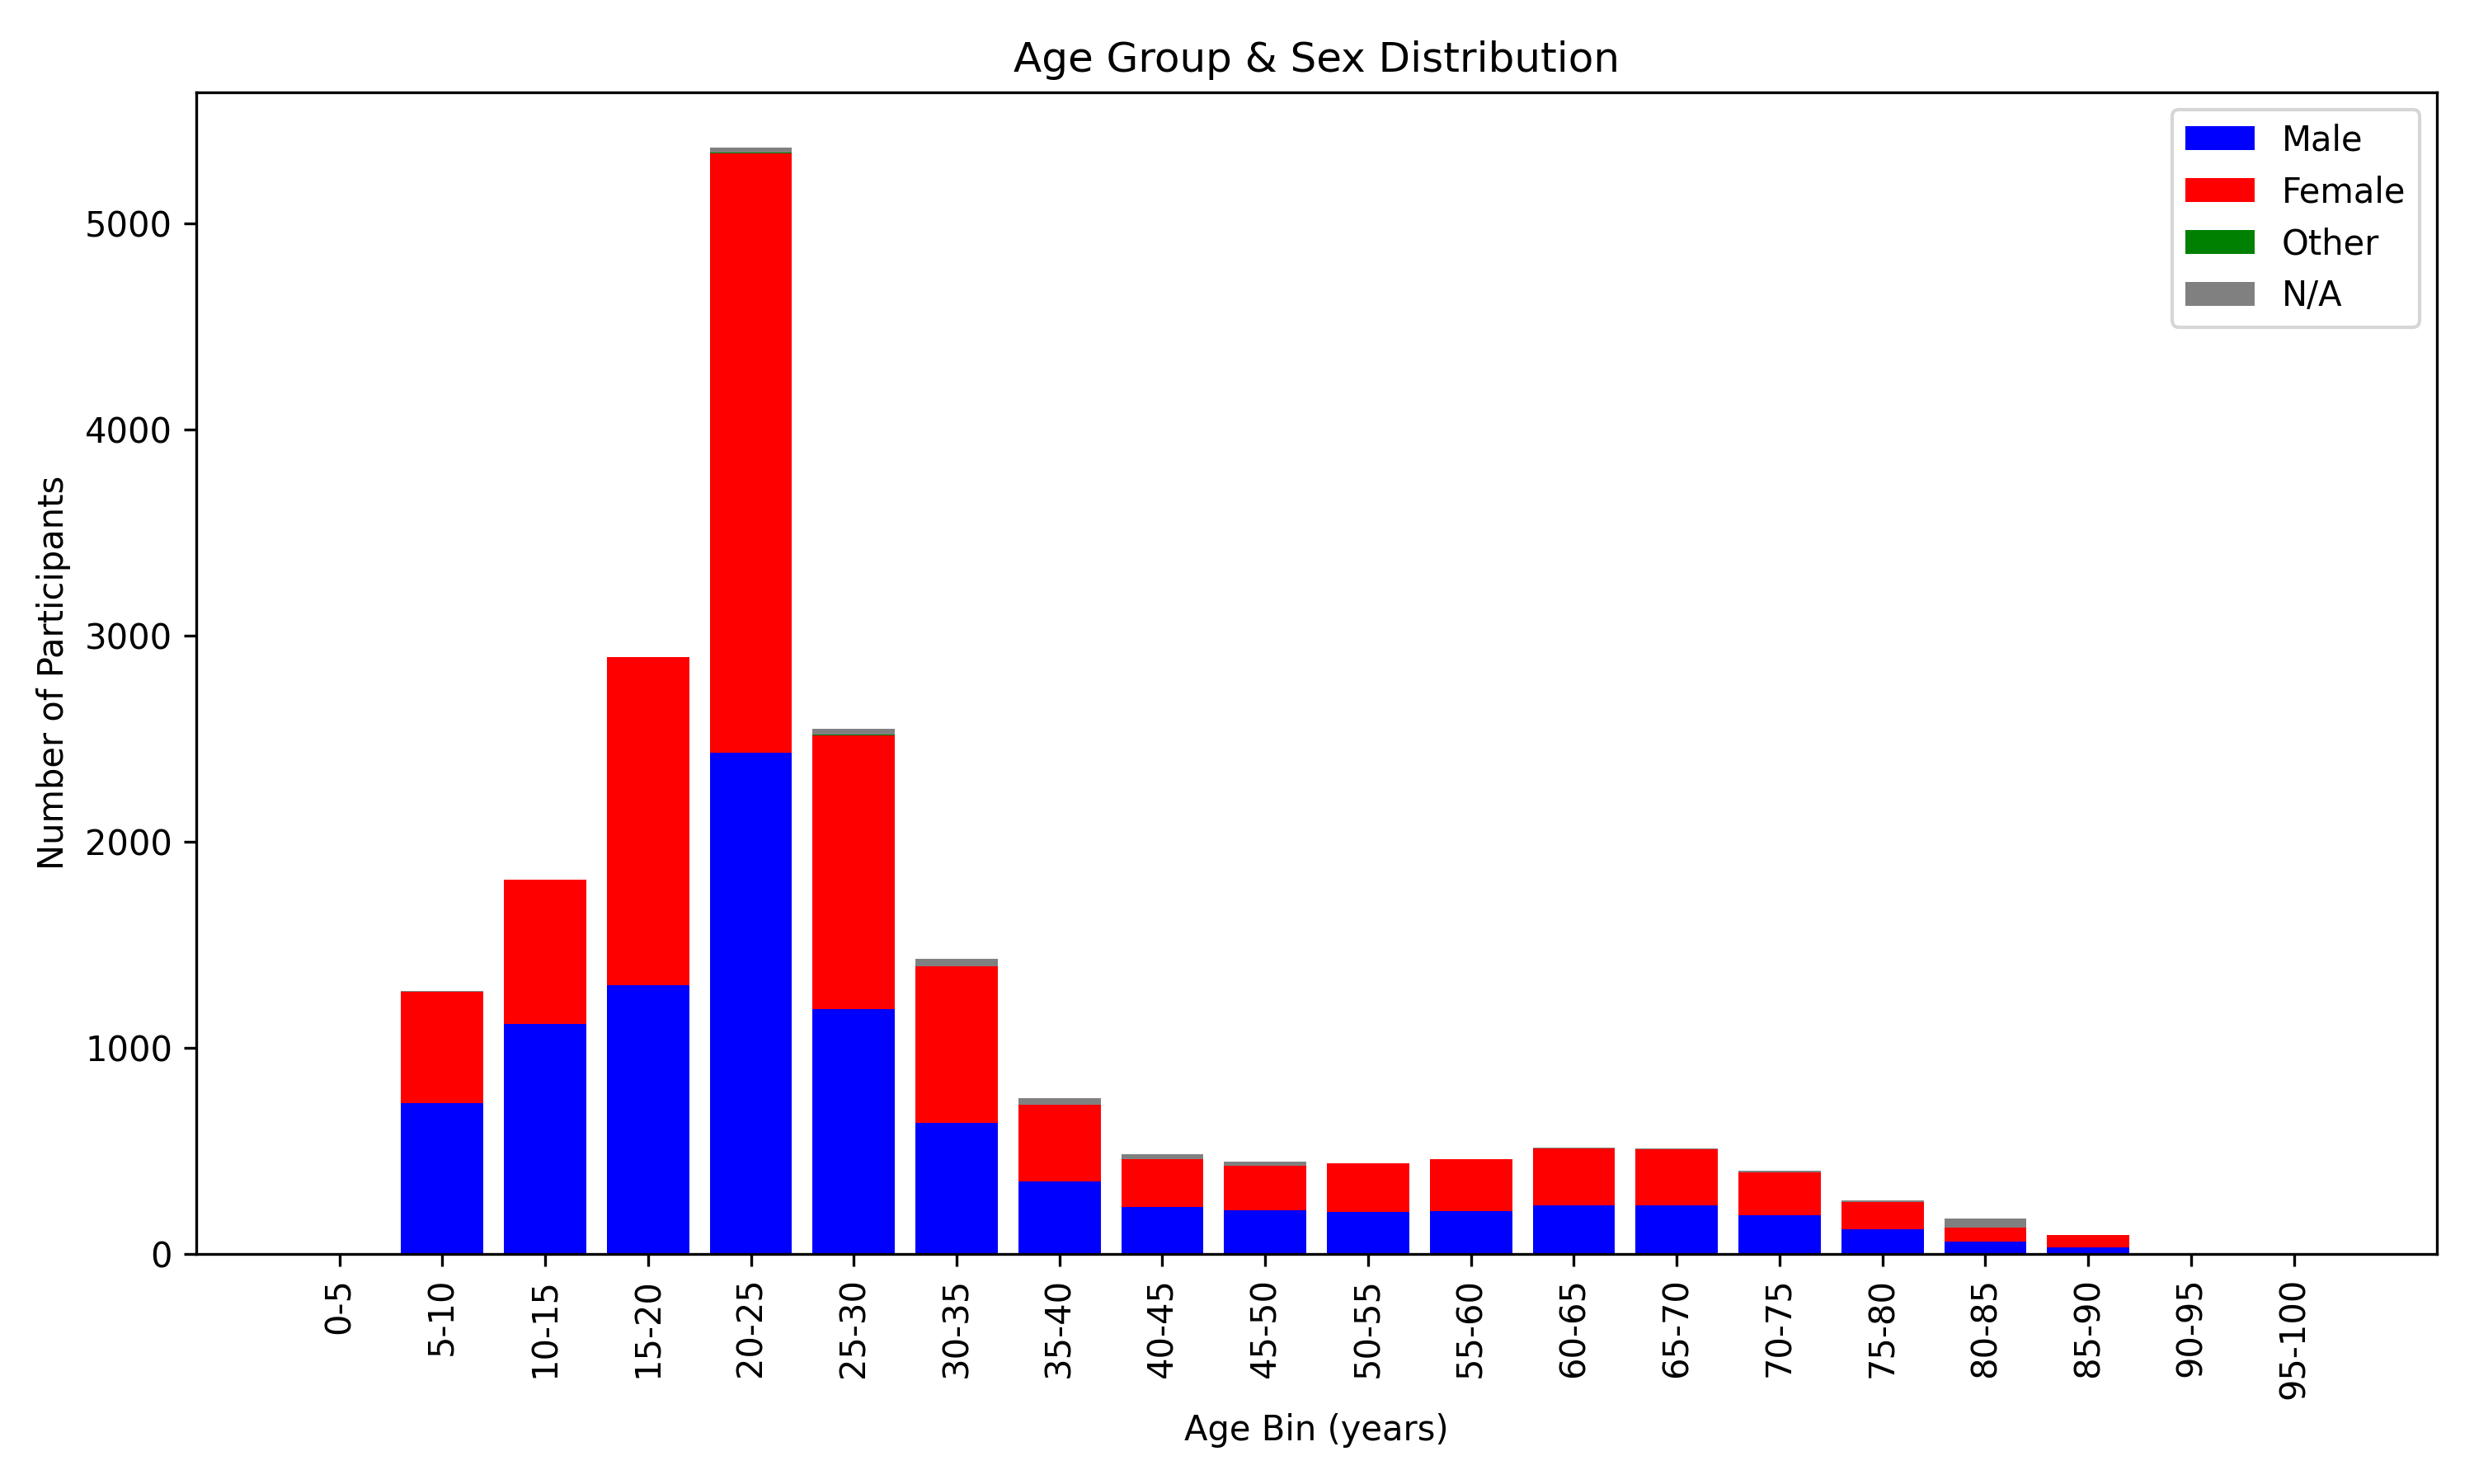
\includegraphics[width=\linewidth]{figures/age_group_sex_histogram} 
    \caption{Histogram of Age (or Age Ranges) by Sex. Each bar represents a bin of age or an age range, subdivided by sex categories (male, female, n/a).}
    \label{HistogramAgeSexFigure}
\end{figure}


\noindent
Figure~\ref{HistogramAgeSexFigure} presents a histogram illustrating how the dataset's age distribution is subdivided by sex categories. 
Specifically, the histogram organizes age (or age range) into bins along the horizontal axis, whereas the vertical bars 
representing the participants count, color-coded to indicate the sex categories: ``male'', ``female'', and ``n/a''. Note: \TotalSubjectsWithSexCountWithoutAgeInfo\ 
subjects who have only sex information and lack age or age range information are omitted from the histogram.


Overall, the mean age (excluding entries with only age range data) is \TotalSubjectsMeanAgeValue\ (SD = \TotalSubjectsStandardDevAgeValue{}). 
By categorizing individual ages into bins, as illustrated in Figure~\ref{HistogramAgeSexFigure}, the median age range is determined to be \TotalSubjectsMedianAgeGroupValue\ years.
The sex distribution among subjects with available sex information, 
regardless of age data, includes \TotalSubjectsWithMaleSexCount\ males 
and \TotalSubjectsWithFemaleCount\ females, 
totaling \TotalSubjectsWithMalePlusFemaleCount\ subjects. 

\begin{table}[ht]
    \centering
    \begin{threeparttable}
        \caption{Distribution of Demographic Variables}
        \label{additional_demographics}
        \begin{tabular}{@{}lcccc@{}}
            \toprule
            \textbf{Variable} & \textbf{Category/Level} & \textbf{Count (n)} & \textbf{Percentage (\%)} & \textbf{Total (n)} \\
            \midrule
            \textbf{Race}   & White & \TotalSubjectsWithWhiteRaceCount & \TotalSubjectsWithWhiteRacePercentage & \TotalSubjectsWithRaceCount \\
                            & Black & \TotalSubjectsWithBlackRaceCount & \TotalSubjectsWithBlackRacePercentage & \\
                            & Asian & \TotalSubjectsWithAsianRaceCount & \TotalSubjectsWithAsianRacePercentage & \\
                            & American Indian/Alaska Native & \TotalSubjectsWithAmericanIndianAlaskanRaceCount & \TotalSubjectsWithAmericanIndianAlaskanRacePercentage & \\
                            & Hawaiian/Pacific Islander & \TotalSubjectsWithHawaiianPacificIslanderRaceCount & \TotalSubjectsWithHawaiianPacificIslanderRacePercentage & \\
                            & Two or More Races & \TotalSubjectsWithTwoOrMoreRaceCount & \TotalSubjectsWithTwoOrMoreRacePercentage & \\
                            & Other & \TotalSubjectsWithOtherRaceCount & \TotalSubjectsWithOtherRacePercentage & \\
            \textbf{Handedness} & Right (R) & \TotalSubjectsWithRightHandednessCount & \TotalSubjectsWithRightHandednessPercentage & \TotalSubjectsWithHandednessCount \\
                                & Left (L) & \TotalSubjectsWithLeftHandednessCount & \TotalSubjectsWithLeftHandednessPercentage & \\
                                & Ambidextrous (A) & \TotalSubjectsWithAmbidextrousHandednessCount & \TotalSubjectsWithAmbidextrousHandednessPercentage &  \\
            \textbf{Education} & Low (Primary/HS) & \TotalSubjectsWithLowEducationCount & \TotalSubjectsWithLowEducationPercentage & \TotalSubjectsWithEducationCount\\ 
                               & Medium (College) & \TotalSubjectsWithMediumEducationCount & \TotalSubjectsWithMediumEducationPercentage & \\
                               & High ($\geq$ Bachelors) & \TotalSubjectsWithHighEducationCount & \TotalSubjectsWithHighEducationPercentage & \\
            \textbf{Socio-Economic Status}  & Low & \TotalSubjectsWithLowEconomicCount & \TotalSubjectsWithLowEconomicPercentage & \TotalSubjectsWithSocioEconomicCount\\
                                            & Medium & \TotalSubjectsWithMediumEconomicCount & \TotalSubjectsWithMediumEconomicPercentage & \\
                                            & High & \TotalSubjectsWithHighEconomicCount & \TotalSubjectsWithHighEconomicPercentage & \\
            \bottomrule
        \end{tabular}
        \begin{tablenotes}[flushleft]\footnotesize
            \item[${a}$] Frequencies and percentages of race, handedness, education, and socio-economic status.
        \end{tablenotes}
    \end{threeparttable}
\end{table}

Beyond age and sex, additional demographic information such as race, handedness, education level, 
and socio-economic status was available only for subsets of participants, 
with notable variability across datasets (see Table~\ref{additional_demographics}). 
Out of \TotalSubjectsWithRaceCount\ subjects with available race information, 
the majority identified as White (\TotalSubjectsWithWhiteRaceCount; \TotalSubjectsWithWhiteRacePercentage\%), 
followed by Black or African American (\TotalSubjectsWithBlackRaceCount; \TotalSubjectsWithBlackRacePercentage\%) 
and Asian (\TotalSubjectsWithAsianRaceCount; \TotalSubjectsWithAsianRacePercentage\%). 
Handedness information, available for \TotalSubjectsWithHandednessCount\ subjects, 
indicated a majority were right-handed (\TotalSubjectsWithRightHandednessCount; \TotalSubjectsWithRightHandednessPercentage\%), 
while left-handed (\TotalSubjectsWithLeftHandednessCount; \TotalSubjectsWithLeftHandednessPercentage\%) 
and ambidextrous (\TotalSubjectsWithAmbidextrousHandednessCount; \TotalSubjectsWithAmbidextrousHandednessPercentage\%) participants were less common.

Educational information for \TotalSubjectsWithEducationCount\ subjects were categorized into three distinct groups: low, medium, and high. 
The low education group (\TotalSubjectsWithLowEducationCount\ subjects, \TotalSubjectsWithLowEducationPercentage\%) includes participants 
who completed primary education or obtained a high school diploma as their highest education level. 
The medium education group (\TotalSubjectsWithMediumEducationCount\ subjects, \TotalSubjectsWithMediumEducationPercentage\%) consists 
of participants who completed some form of post-secondary education below a four-year degree, such as college, a diploma, or an Associate's Degree. 
The high education category (\TotalSubjectsWithHighEducationCount\ subjects, \TotalSubjectsWithHighEducationPercentage\%) comprises individuals 
who have completed at least a Bachelor's degree, including Master's or doctoral degrees (PhD). 
Similarly, socioeconomic status, available for \TotalSubjectsWithSocioEconomicCount\ subjects, is categorized into 
low (\TotalSubjectsWithLowEconomicCount\ subjects, \TotalSubjectsWithLowEconomicPercentage\%), 
medium (\TotalSubjectsWithMediumEconomicCount\ subjects, \TotalSubjectsWithMediumEconomicPercentage\%), and high (\TotalSubjectsWithHighEconomicCount\ subjects, 
\TotalSubjectsWithHighEconomicPercentage\%) groups.

% Educational information for \TotalSubjectsWithEducationCount\ subjects were categorized into three distinct groups: low, medium, and high. 
% The \textit{low} education group (\TotalSubjectsWithLowEducationCount\ subjects, \TotalSubjectsWithLowEducationPercentage\%) includes participants 
% who completed primary education or obtained a high school diploma as their highest education level. 
% The \textit{medium} education group (\TotalSubjectsWithMediumEducationCount\ subjects, \TotalSubjectsWithMediumEducationPercentage\%) consists 
% of participants who completed some form of post-secondary education below a four-year degree, such as college without degree completion, a diploma, or an Associate's Degree. 
% The \textit{high} education category (\TotalSubjectsWithHighEducationCount\ subjects, \TotalSubjectsWithHighEducationPercentage\%) comprises individuals 
% who have completed at least a Bachelor's degree, including Master's or doctoral degrees (PhD). 


\subsubsection{Participants from clinical cohorts}

A total of \TotalSubjectsWithDisordersCount\ participants that are part of the BrainScape dataset have been diagnosed with disorders.
These disorders include Neurological disorders (Stroke, Prosopagnosia, Dysembryoplastic Neuroepithelial Tumor(DNT), Gliosis, and Epilepsy), Psychiatric disorder (Depression, and Schizophrenia)
and Developmental disorder (Attention-Deficit/Hyperactivity Disorder(ADHD) and Autism Spectrum Disorder (ASD)). 
Table~\ref{brain_disorders} lists the number of subjects diagnosed with each disorder among 
the overall \TotalSubjectsIncludedAfterInspectionCount\ individuals. 


\begin{table}[ht]
    \centering
    \begin{threeparttable}
        \caption{Number of Subjects with specific Disorders}
        \label{brain_disorders}
        \begin{tabular}{@{}lc@{}}
            \toprule
            \textbf{Disorder} & \textbf{Number of Subjects} \\
            \midrule
            Stroke & \SubjectsWithStrokeCount\ \\
            Acute Ischemic Stroke & \SubjectsWithAcuteIschemicStrokeCount\ \\
            Schizophrenia & \SubjectsWithSchizophreniaCount\ \\
            Depression & \SubjectsWithDepressionCount\ \\
            ADHD & \SubjectsWithADHDCount\ \\
            ASD & \SubjectsWithASDCount\ \\
            Bipolar Disorder & \SubjectsWithBIPOLARCount\ \\
            Prosopagnosia & \SubjectsWithProsopagnosiaCount\ \\
            Epilepsy & \SubjectsWithEpilepsyCount\ \\
            Focal Epilepsy & \SubjectsWithFocalEpilepsyCount\ \\
            Tumor & \SubjectsWithTumorCount\ \\
            Gliosis & \SubjectsWithGLCount\ \\           
            DNT & \SubjectsWithDNTCount\ \\
            Aneurysm & \SubjectsWithAneurysmCount\ \\
            \bottomrule
        \end{tabular}
        \begin{tablenotes}[flushleft]\footnotesize
            \item[${a}$] Only participants who tested \texttt{Y} (Yes) for each disorder are counted here.
        \end{tablenotes}
    \end{threeparttable}
\end{table}

% \begin{table}[ht]
%     \centering
%     \begin{threeparttable}
%         \caption{Number of Subjects with specific Disorders}
%         \label{brain_disorders}
%         \begin{tabular}{@{}lc@{}}
%             \toprule
%             \textbf{Disorder} & \textbf{Number of Subjects} \\
%             \midrule
%             Stroke & \SubjectsWithStrokeCount\ \\
%             Schizophrenia & \SubjectsWithSchizophreniaCount\ \\
%             Depression & \SubjectsWithDepressionCount\ \\
%             ADHD & \SubjectsWithADHDCount\ \\
%             ASD & \SubjectsWithASDCount\ \\
%             Bipolar Disorder & \SubjectsWithBIPOLARCount\ \\
%             Prosopagnosia & \SubjectsWithProsopagnosiaCount\ \\
%             Epilepsy & \SubjectsWithEpilepsyCount\ \\
%             Tumor & \SubjectsWithTumorCount\ \\
%             Acute Ischemic Stroke & \SubjectsWithAcuteIschemicStrokeCount\ \\
%             Focal Epilepsy(Focal Cortical Dysplasia) & \SubjectsWithFCDCount\ \\
%             Focal Epilepsy(Hippocampal Sclerosis) & \SubjectsWithHSCount\ \\
%             DNT & \SubjectsWithDNTCount\ \\
%             Gliosis & \SubjectsWithGLCount\ \\
%             Aneurysm & \SubjectsWithAneurysmCount\ \\
%             \bottomrule
%         \end{tabular}
%         \begin{tablenotes}[flushleft]\footnotesize
%             \item[${a}$] Only participants who tested \texttt{Y} (Yes) for each disorder are counted here.
%         \end{tablenotes}
%     \end{threeparttable}
% \end{table}


\noindent
Table~\ref{brain_disorders} highlights that \SubjectsWithStrokeCount\ participants have been 
diagnosed with stroke, \SubjectsWithEpilepsyCount\ with epilepsy, and so on. 
The \SubjectsWithFocalEpilepsyCount\ subjects with focal epilepsy consist of \SubjectsWithFCDCount\ subjects 
with focal cortical dysplasia and \SubjectsWithHSCount\ subjects with hippocampal sclerosis.
In total, \TotalSubjectsWithDisordersCount\ participants have at least one neurological, psychiatric, or developmental disorder.



\subsubsection{Quality Control and Visual Inspection}

All MRI datasets included in this study underwent visual inspection to identify and exclude scans presenting various artifacts, 
including motion artifacts, susceptibility distortions, aliasing (wrap-around) artifacts, and Gibbs ringing artifacts. 
Similarly, subjects with poorly defaced MRIs, where portions of the brain were inadvertently removed, were excluded. For transparency and 
traceability, any scan failing visual quality checks is listed in the corresponding dataset's metadata, enabling researchers to audit, 
revisit, or reverse these exclusions if required.

This process has thus far resulted in the removal of \TotalNumSubjectsRemoved\ subjects across \TotalNumDatasetsWithSubjectsRemoved\ datasets 
from the total of \NumDatasets\ included in the repository. 
Additionally, \NumDatasetsAlreadySkullStripped\ datasets out of the total \NumDatasets\ have brain MRIs that were already skull-stripped. 
However, we opted to exclude scans with incomplete skull stripping, such as those illustrated in Figure \ref{dropped_subject}. 
Reprocessing datasets that contain both fully and partially skull-striped MRIs with the default BraTS preprocessing plugin, 
which uses HD-BET brain-extraction tool (\cite{isensee2019automated}) results in over-erosion of brain tissue during brain extraction.
We decided to drop incomplete skull stripped scans from such datasets to keep a single default BraTS preprocessing pipeline for the BrainScape dataset release, 
and because this issue affected only a small subset of subjects (approximately 130 subjects).
Figure~\ref{dropped_subject} illustrates examples of the excluded MRI scans, highlighting the types of artifacts and issues that led to their removal. By making the exclusion 
criteria explicit and open to re-evaluation by the neuroscience community, we reduce the risk of perpetuating errors and encourage collaborative quality assurance, 
ultimately enhancing the overall integrity and reproducibility of the dataset.


\begin{figure}[htbp]\begin{center}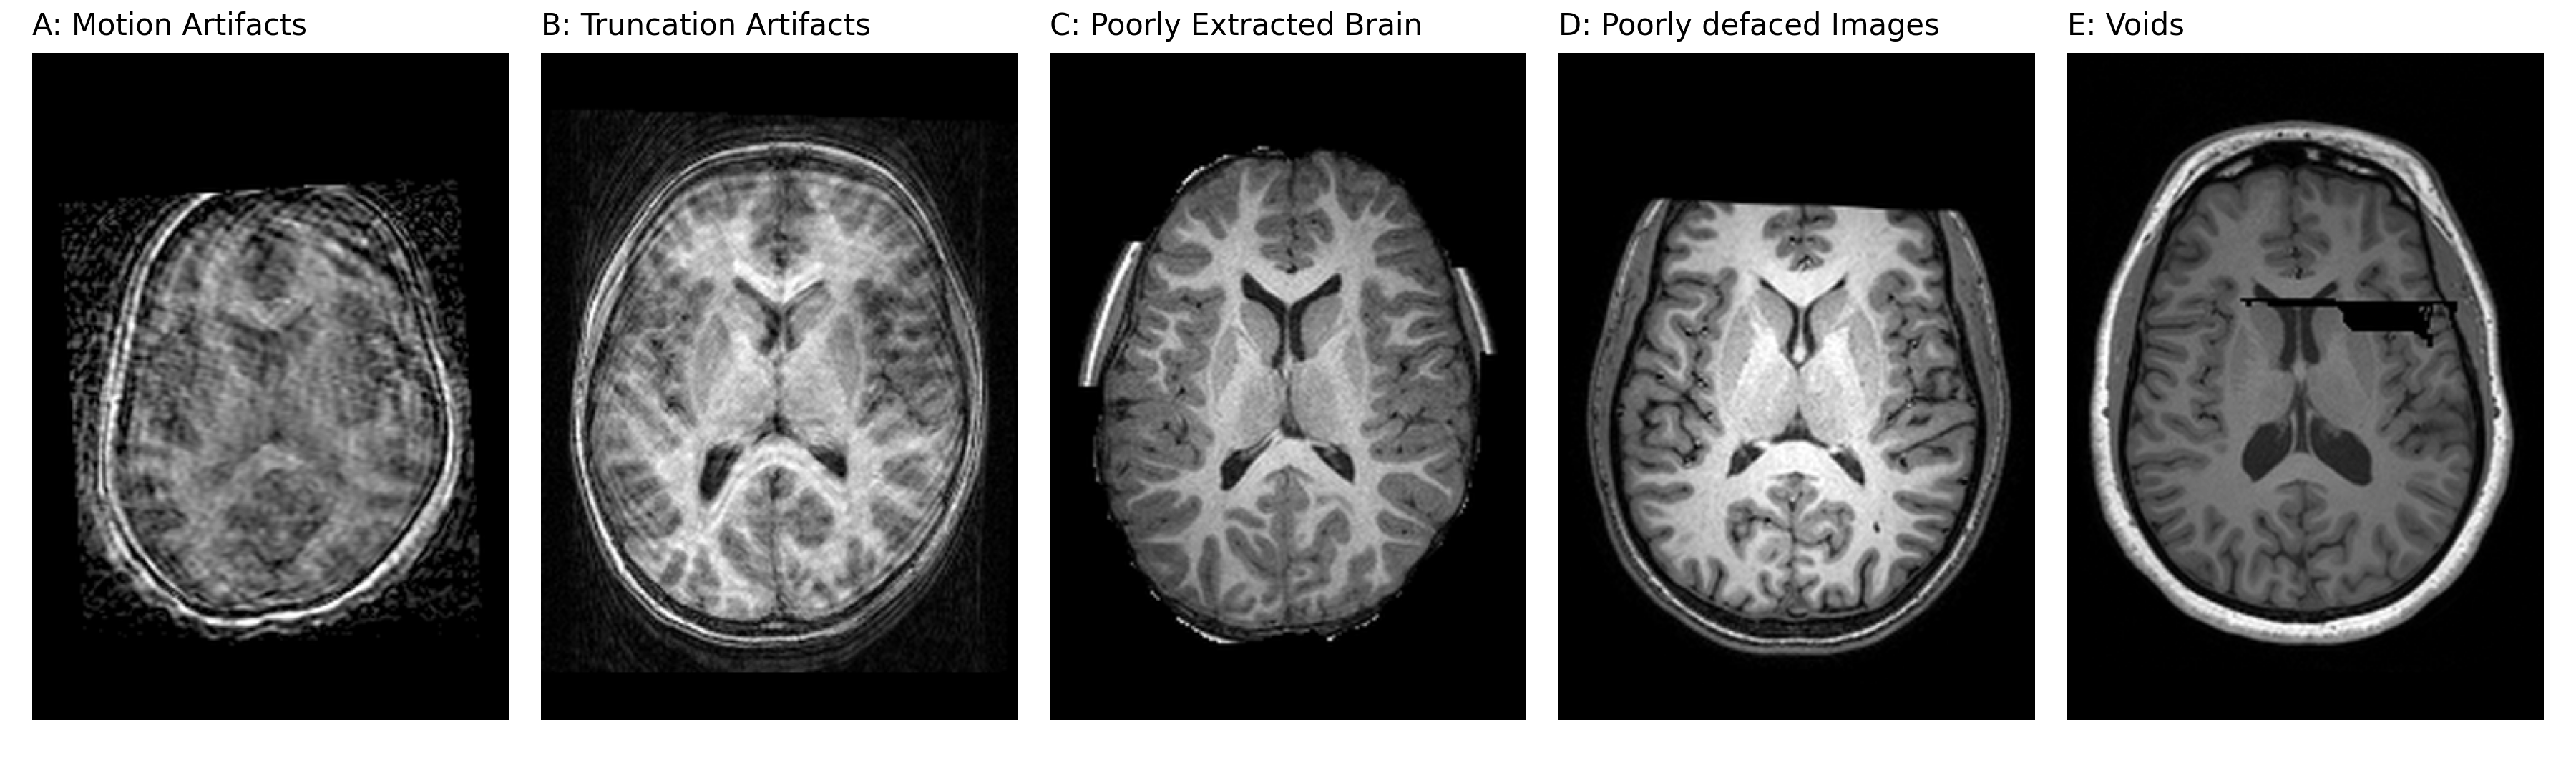
\includegraphics[width=\linewidth]{figures/dropped_subjects.png}
    \caption{
        Examples of MRI scans excluded during visual quality inspection:
        (A) Motion artifacts, 
        (B) Gibbs ringing artifact (truncation artifact), 
        (C) Poorly extracted brain regions, 
        (D) Inadequate defacing with cropped brain regions, 
        and (E) Missing or void pixels.
    }
    \label{dropped_subject}\end{center}
\end{figure}


\subsection{Computational Performance and Carbon Footprint}

The BrainScape framework completed the full workflow for the VASP dataset (120 MRI scans) in approximately 33.3\,minutes of wall-clock time. 
The recorded CPU utilization was only 21.85\%, reflecting the predominantly sequential structure of our current implementation. 
In total, the pipeline took 228\,minutes of CPU time across the 24 CPU cores, indicating further room for parallelization. 
Future updates to BrainScape are expected to enable running multiple datasets concurrently, 
which can significantly shorten wall-clock time and increase overall efficiency.
Real-time monitoring of GPU resources revealed that usage peaked during skull stripping (during preprocessing), 
with memory consumption reaching about 5406\,MB (44\% of the available 12\,GB). 
Outside of these intensive operations, the GPU remained largely idle, resulting in an average utilization 
of 24.78\% throughout the entire workflow. 
Incorporating additional datasets is expected to proportionally increase wall-clock time and CPU time.

We also evaluated the pipeline's environmental impact by considering local grid emission factors in New Zealand. 
Over the entire run on the VASP dataset, the pipeline consumed an estimated 0.07065 kilowatt-hours (kWh) of electricity, corresponding to 
0.00796\,kg of CO\textsubscript{2}eq emissions. 
0.07065 kWh is roughly the energy needed to keep a 10 W LED lamp on for seven hours, 
or to run a typical 1.5 kW space heater for a little under three minutes.
As more datasets are included, the energy consumption and 
carbon footprint may rise proportionally; however, workflow parallelization can help maintain 
reasonable total run times and minimize ecological impact. By documenting these performance metrics, we highlight 
the computational overhead and the opportunity to reduce processing times and emissions through concurrent dataset handling. 
We anticipate that implementing parallel dataset processing pipelines will improve BrainScape's computational performance and carbon footprint.


